在FPGA上运行内核有两个步骤(与提前编译一样):\par

\begin{enumerate}
	\item 将源代码编译成二进制文件,可以在感兴趣的硬件上运行
	\item 运行时选择感兴趣的加速器
\end{enumerate}

为了编译内核在FPGA硬件上运行,可以使用命令行:\par

\begin{tcolorbox}[colback=white,colframe=black]
dpcpp -fintelfpga my\_source\_code.cpp -Xshardware
\end{tcolorbox}

这个命令告诉编译器将my\_source\_code.cpp中的所有内核转换为可以在Intel FPGA加速机上运行的二进制文件,然后打包到主机二进制文件中。当执行主机二进制文件时(例如,在Linux上运行./a.out),在执行提交的内核之前,运行时将根据需要为FPGA自动编程,如图17-8所示。\par

\hspace*{\fill} \par %插入空行
图17-8 FPGA在运行时的自动编程
\begin{center}
	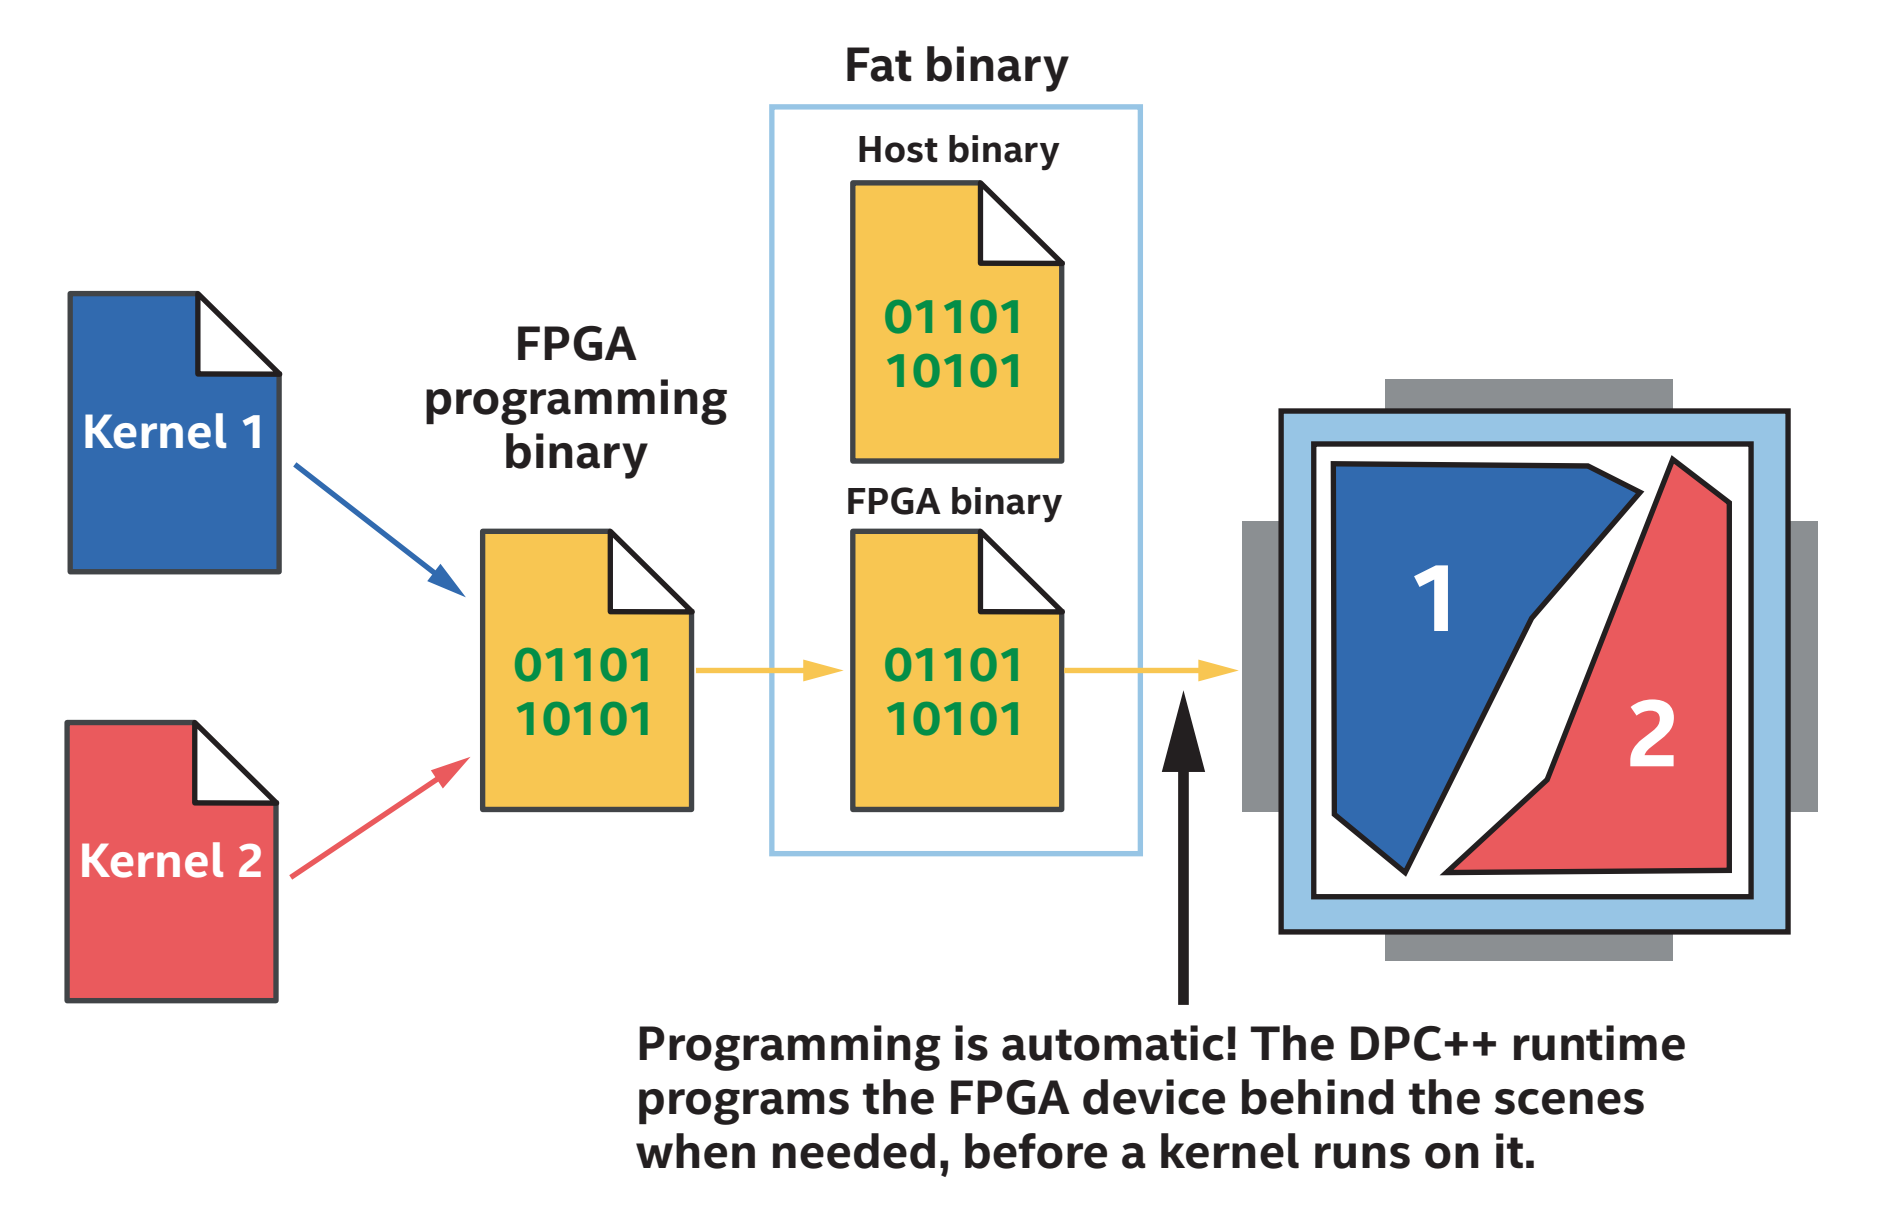
\includegraphics[width=1.0\textwidth]{content/chapter-17/images/9}
\end{center}

\begin{tcolorbox}[colback=red!5!white,colframe=red!75!black]
FPGA编程二进制文件嵌入在主机上运行和编译的DPC++可执行文件中。FPGA在后台进行自动配置。\\

当运行主程序并在FPGA上提交内核执行时,在内核开始执行之前可能会有一个延迟。重新提交内核执行不会出现相同的延迟,因为内核已经编程到设备中,并准备运行。
\end{tcolorbox}

运行时选择FPGA设备在第2章中讨论。需要告诉主程序希望内核在哪里运行,通常会有多个加速器选项可用,比如CPU和GPU,除了FPGA。为了快速回顾在程序执行期间选择FPGA的方法,可以使用如图17-9所示的代码。\par

\hspace*{\fill} \par %插入空行
图17-9 使用fpga\_selector在运行时选择FPGA
\begin{lstlisting}[caption={}]
#include <CL/sycl.hpp>
#include <CL/sycl/intel/fpga_extensions.hpp> // For fpga_selector
using namespace sycl;

void say_device (const queue& Q) {
	std::cout << "Device : "
			  << Q.get_device().get_info<info::device::name>() 
			  << "\n";
}

int main() {
	queue Q{ INTEL::fpga_selector{} };
	say_device(Q);
	
	Q.submit([&](handler &h){
		h.parallel_for(1024, [=](auto idx) {
			// ...
		});
	});

	return 0;
}
\end{lstlisting}

\hspace*{\fill} \par %插入空行
\textbf{编译时间}

很多传言说,为FPGA编译设计可能需要很长时间,比基于ISA的加速器编译时间长得多。传言是真的!本章的最后概述了FPGA的细粒度架构元素,它们带来了FPGA的优点和计算密集型的编译(位置和路径优化),在某些情况下需要花费数小时。\par

从源代码到FPGA硬件执行的编译时间足够长,以至于我们不希望只在硬件中开发和迭代代码。FPGA开发流程提供了几个阶段,这些阶段最小化了硬件编译的数量,使硬件编译的时间不受影响时,仍然具有生产力。图17-10显示了典型的阶段,大部分时间都花在提供快速周转和快速迭代的早期步骤上。\par

\hspace*{\fill} \par %插入空行
图17-10 大多数验证和优化发生在冗长的硬件编译之前
\begin{center}
	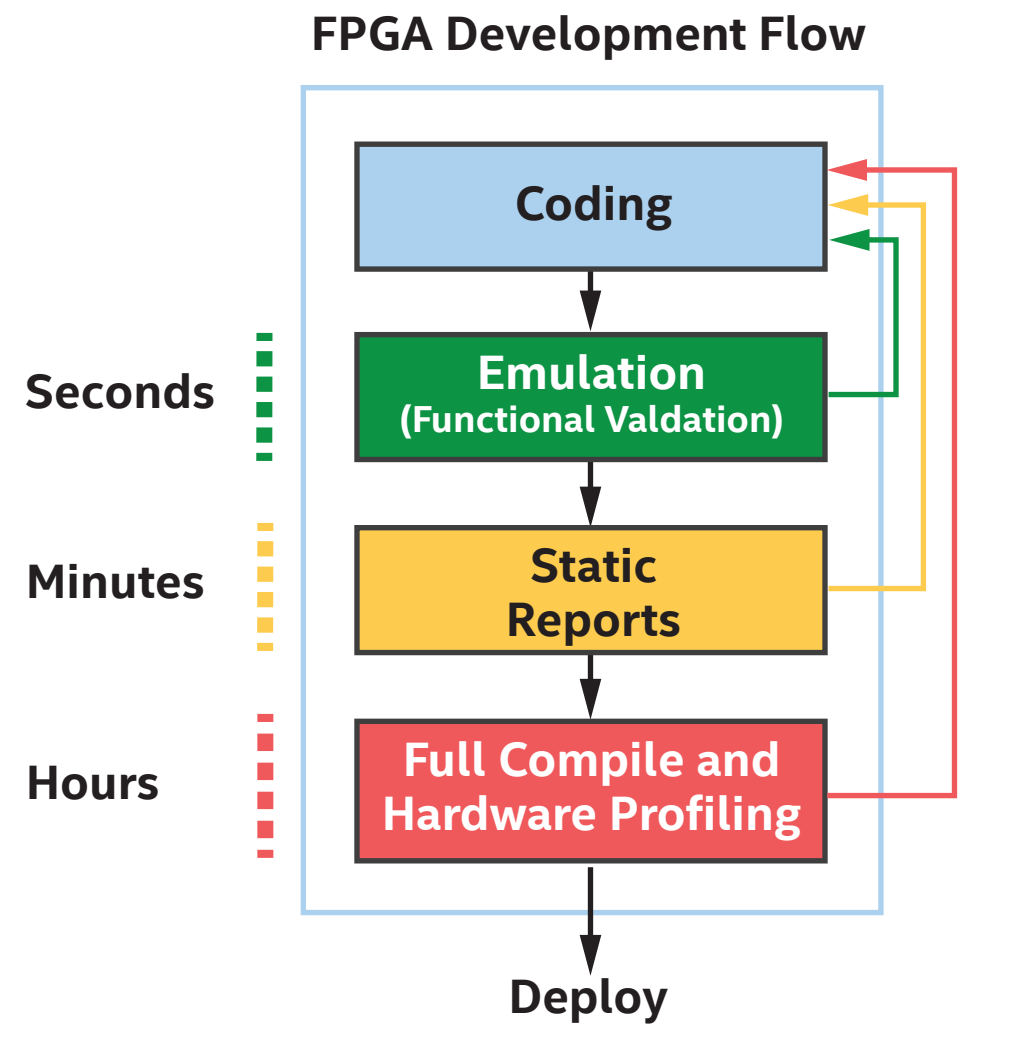
\includegraphics[width=0.6\textwidth]{content/chapter-17/images/10}
\end{center}

编译器的渲染和静态报告是DPC++中FPGA代码开发的基石。模拟器支持相关的扩展和执行模型,在主机上运行。因此,编译时间与期望从编译到CPU设备的时间相同,尽管看不到在实际FPGA硬件上执行所带来的性能提升。模拟器对于在应用程序中建立和测试功能正确性非常有用。\par

工具链可以快速生成静态报告,比如仿真。报告由编译器创建的FPGA结构,并由编译器识别的瓶颈。这两者都可以用来预测设计在FPGA硬件上运行时是否会有良好的性能,并用于优化代码。请阅读供应商的文档以获取有关报告的信息,这些报告通常会随着工具链的发布而不断改进(请参阅文档以获得最新和最伟大的特性!)供应商提供了详细的文档,说明如何根据报告进行解释和优化。这些信息将是另一本书的主题,所以不在这一章中详细讨论。\par

\hspace*{\fill} \par %插入空行
\textbf{FPGA仿真器}

模拟主要用于从功能上调试应用程序,以确保它的行为符合预期并产生正确的结果。没有理由在编译时间较长的实际FPGA硬件上进行这种级别的开发。仿真流通过从dpcpp编译命令中删除-Xshardware标志来激活,并且在我们的主机代码中使用INTEL::fpga\_emulator\_selector,而不是使用INTEL::fpga\_selector。然后,使用以下命令进行编译\par

\begin{tcolorbox}[colback=white,colframe=black]
dpcpp -fintelfpga my\_source\_code.cpp
\end{tcolorbox}

同时,将在运行时使用如图17-11所示的FPGA仿真器。通过使用FPGA模拟器选择器(使用主机处理器来模拟FPGA),需要对实际的FPGA硬件进行冗长的编译之前,维护一个快速的开发和调试过程。\par

\hspace*{\fill} \par %插入空行
图17-11 利用FPGA仿真器进行快速开发和调试
\begin{lstlisting}[caption={}]
#include <CL/sycl.hpp>

#include <CL/sycl/intel/fpga_extensions.hpp> // For fpga_selector
using namespace sycl;

void say_device (const queue& Q) {
	std::cout << "Device : "
			  << Q.get_device().get_info<info::device::name>() << "\n";
}

int main() {
	queue Q{ INTEL::fpga_emulator_selector{} };
	say_device(Q);
	
	Q.submit([&](handler &h){
		h.parallel_for(1024, [=](auto idx) {
			// ...
			});
		});

	return 0;
}
\end{lstlisting}

如果经常在硬件和模拟器之间切换,可以在程序中使用宏在对设备选择器进行切换。如果需要,请查看供应商的文档和在线FPGA DPC++代码示例。\par

\hspace*{\fill} \par %插入空行
\textbf{FPGA的AOT(Ahead-of-Time)编译}

图17-10中的完全编译和硬件分析阶段在SYCL术语中是AOT编译。意味着将内核编译为设备二进制文件,是发生在最初编译程序时,而不是在将程序提交给要运行的设备时。在FPGA上,这一点特别重要,因为\par

\begin{enumerate}
	\item 编译需要一段时间,这是运行程序时不希望发生的。
	\item DPC++程序可能会在没有主机处理器的系统上执行。FPGA二进制代码的编译过程得益于快速处理器和大量附加内存。AOT编译可以轻松地选择编译发生的位置,而不是让它在部署程序的系统上运行。
\end{enumerate}

\begin{tcolorbox}[colback=blue!5!white,colframe=blue!75!black, title=在FPGA上使用DPC++其实要经历很多!]
传统的FPGA设计(不使用高级语言)可能非常复杂。除了编写内核之外,还有许多步骤,比如:构建和配置与芯片外存储器通信的接口,通过插入寄存器来关闭计时,这些寄存器需要使编译后的设计运行得足够快,以便与某些外设通信。DPC++解决了这一切,所以不需要知道任何关于传统FPGA设计的细节来实现工作应用程序!该工具将内核当作代码来优化和提高设备效率,然后自动处理与芯片外外设通信、关闭计时和设置驱动程序的所有细节。\\

与任何其他加速器一样,要在FPGA上实现峰值性能仍然需要详细的架构知识,但使用DPC++从代码转移到工作设计的步骤,比传统FPGA流程要简单得多,生产率也更高。
\end{tcolorbox}



















